\section{Experiments}
\label{sec-1}
\subsection{Results}
\label{sec-1-1}
\begin{frame}[label=sec-1-1-1]{Accuracy convergance}
\begin{minipage}{0.55\linewidth} 
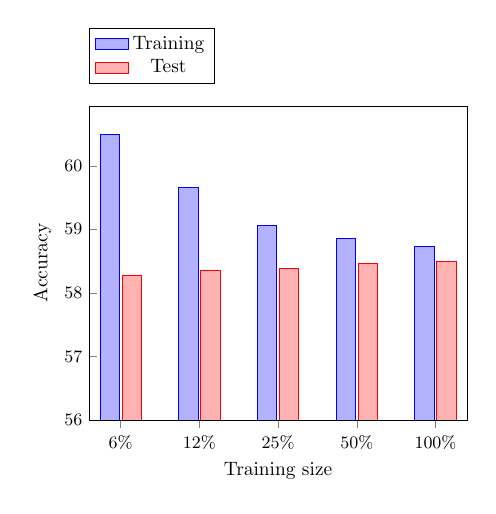
\begin{tikzpicture}[scale=0.70]
\begin{axis}[
ybar,
ylabel = Accuracy,
xlabel = Training size,
tick label style={font=\small},
tickpos=left,
xticklabels={6\%, 12\%, 25\%, 50\%, 100\%}, 
xtick={1,2,3,4,5, 6},
ymin=56,
legend entries={Training,Test},
legend style={at={(0.165,1.25)}, anchor=north,legend columns=1},
legend image code/.code={\draw[#1] (0cm,-0.1cm) rectangle (0.6cm,0.1cm);},   
]   
\addplot +[bar shift=-.2cm] coordinates {(1,60.49) (2,59.66) (3,59.06) (4,58.85) (5,58.73)  };
\addplot +[bar shift=.2cm]coordinates {(1,58.28) (2,58.36) (3,58.38) (4, 58.46) (5,58.50) };
\end{axis}
\end{tikzpicture}
\end{minipage}
\begin{minipage}{0.40\linewidth} 
\begin{itemize}
\item All prematch features
\item Logistic regression
\item Stochastic gradient descent 
\item L2-regularisation (regularisation factor of 0.01)
\end{itemize}
\vspace{0.05cm}
\begin{itemize}
\item Increased test data size gives no visible benefit
\item Increased training data size lowers overfitting
\end{itemize}
\end{minipage}
\end{frame}

\begin{frame}[label=sec-1-1-2]{Feature experiments}
\begin{minipage}{0.55\linewidth} 
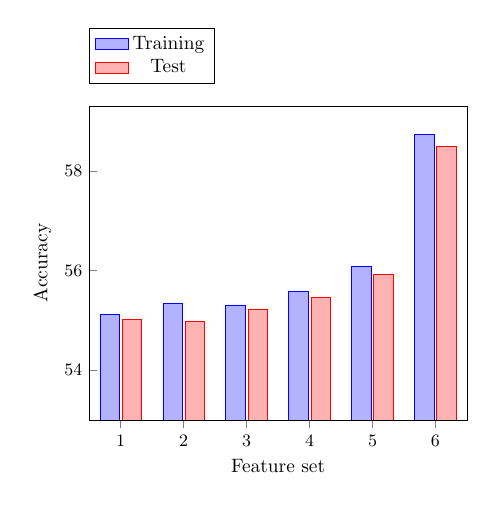
\begin{tikzpicture}[scale=0.70]
\begin{axis}[
ybar,
ylabel = Accuracy,
xlabel = Feature set,
tick label style={font=\small},
tickpos=left,
xticklabels={1, 2, 3, 4, 5, 6}, 
xtick={1,2,3,4,5, 6},
ymin=53,
legend entries={Training,Test},
legend style={at={(0.165,1.25)}, anchor=north,legend columns=1},
legend image code/.code={\draw[#1] (0cm,-0.1cm) rectangle (0.6cm,0.1cm);},   
]   
\addplot +[bar shift=-.2cm] coordinates {(1,55.12) (2,55.34) (3,55.31)  (4,55.58)     (5,56.08) (6, 58.73)};

\addplot +[bar shift=.2cm]coordinates {(1,55.01) (2,54.98) (3,55.22) (4,  55.46) (5,55.92) (6, 58.50)};

\end{axis}
\end{tikzpicture}
\end{minipage}    
\begin{minipage}{0.40\linewidth}
\footnotesize{
\begin{enumerate}
\item $\phi_\text{SINGLE}$
\item $\phi_\text{PAIR}$
\item $\phi_\text{SINGLE}$, $\phi_\text{PAIR}$
\item $\phi_\text{SINGLE}$, $\phi_\text{PAIR}$, $\phi_\text{COUNTER}$
\item $\phi_\text{SINGLE}$, $\phi_\text{PAIR}$, $\phi_\text{COUNTER}$, $\phi_\text{BEST-RANK}$
\item $\phi_\text{SINGLE}$, $\phi_\text{PAIR}$, $\phi_\text{COUNTER}$, $\phi_\text{BEST-RANK}$, $\phi_\text{PLAYER-RANK}$, $\phi_\text{LANE-RANKS}$, $\phi_\text{LANE-CHAMPION}$, $\phi_\text{CHAMPION-SPELLS}$, $\phi_\text{CHAMPION-RUNES}$, $\phi_\text{CHAMPION-MASTERIES}$
\end{enumerate}
}
\end{minipage}
\end{frame}


\subsection{Knowledge extraction}
\label{sec-1-2}
\begin{frame}[label=sec-1-2-1]{Accuracy}
\begin{itemize}
\item Reasons for low accuracy:
\begin{itemize}
\item Features not thoroughly  representative
\item Highest accuracy achieved
\end{itemize}
\item Combination of features:
\begin{itemize}
\item Accuracy not better when rank based features are combined
\item Different features does cause better accuracy
\end{itemize}
\end{itemize}
\end{frame}

\begin{frame}[label=sec-1-2-2]{Notable weights}
\begin{itemize}
\item No weights that standout by a lot
\item Mostly symmetric around 0
\end{itemize}
\vspace{0.05}
\begin{itemize}
\item Negative for Blue:
\begin{itemize}
\item Jinx-BLUE-VS-LeeSin-PURPLE
\item Blitzcrank-BLUE-VS-LeeSin-PURPLE
\end{itemize}
\item Positive for Blue:
\begin{itemize}
\item LeeSin-BLUE-VS-Blitzcrank-PURPLE
\end{itemize}
\item Possible reason:
\begin{itemize}
\item Blitzcrank can pull enemies in
\item LeeSin can jump away
\end{itemize}
\end{itemize}
\end{frame}
\subsection{Conclusion}
\label{sec-1-3}
\begin{frame}[label=sec-1-3-1]{Conclusion}
\begin{itemize}
\item Worked with large dataset of 456GB
\item Cluster of 4 machines, 3 workers and 1 master running HDFS and Apache spark
\item Best accuracy achieved is 58.5\% using logistic regression
\begin{itemize}
\item Most likely as a consequence of balanced game
\end{itemize}
\item Results can be used for a tool that helps LoL players pick a winning champion or team
\end{itemize}
\end{frame}
\begin{frame}[label=sec-1-3-2]{Future work}
\begin{itemize}
\item Add additional features
\item If size of cluster is increased, better fault tolerance could be added
\item Evaluation of a game while it is going on
\begin{itemize}
\item This would increase the number of features by a lot
\item Based on events happening in the game, e.g. the dragon getting killed
\end{itemize}
\item An agent that could play optimally
\end{itemize}
\end{frame}